\chapter{Entrada e Saída}

Para prover um abstração simples da máquina física, o sistema operacional deve conhecer bem cada \textit{hardware} sobre o qual ele opera, uma vez que cada um destes dispositivos tem um conjunto de comandos específicos. Unidades de E/S são compostas de uma parte mecânica, que é o dispositivo, e uma parte eletrônica, que é a sua controladora.

Em geral, dividem-se dispositivos de entrada e saída em dois tipos:
\begin{itemize}
  \item \textbf{Dispositivos de Bloco:} onde temos informações sendo armazenadas em unidades de tamanho fixo e sua recuperação é feita por acesso direto. \underline{Exemplo:} disco rídigo;

  \item \textbf{Dispositivos de Caractere:} a informação é aceita em unidadades de tamanho variável, Geralmente sendo armazenada temporariamente ou não sendo armazenada. \underline{Exemplo:} terminais, impressoras, \textit{mouse}, etc..
\end{itemize}

\textbf{O SO programa a controladora}. Ambos trocam informações constantemente, por meio de registradores, sendo estes geralmente são mapeados em posições fixas de memória. O SO solicita alguma entrada ou saída escrevendo nestes registradores.

Cada controladora tem um conjunto de comandos específicos de baixo nível, que são descritos em seus manuais. Uma vez aceito o comando, a controladora trabalha simultaneamente com a CPU, somente interrompendo-a no final do serviço.







\section{\textit{Software de E/S}}
A maioria dos sistemas operacionais modernos utiliza o conceito de indepêndencia de dispositivos. Além disso, é importante haver \textbf{uniformidade da indentificação}, ou seja, o nome de um dispositivo lógico ou de um arquivo não deve depender do dispositivo físico ao qual está associado no momento.

\begin{definicao}{Independência de Dispositivos}
  Execução de um mesmo programa com dispositivos físicos diferentes.
\end{definicao}

\textit{Softwares} de E/S podem ser estruturados em: manipuladores de interrupção, \textit{drivers} de dispositivo, SO independente de dispositivo e aplicações de usuário.





\subsection{Manipuladores de Interrupção}
As operações de E/S podem ser tratadas de maneira síncrona ou assíncrona. A maioria dos SO tradicionais as trata de maneira síncrona, ou seja, o processo que solicitou uma operação de E/S fica bloqueado até que esta operação se complete.

Dessa forma, o SO tradicional pode tratar várias operações ao mesmo tempo, porém somente uma interrupção por processo pode estar sendo tratada. Quando ocorre um interrupção, isto indica que a operação se completou e o SO coloca o processo, que estava bloqueado, na fila \textit{ready}.

\textbf{Nota:} as manipulações de interrupção devem ser feitas e modo protegido.




\subsection{\textit{Drivers} de Dispositivo}
O \textit{driver} de dispositivo é a parte do SO que executa código dependente de \textit{hardware} do dispositivo, onde cada um destes possui seu \textit{driver} específico. O \textit{driver} recebe solicitações abstratas e as traduz para comandos específicos.

No caso do disco rígido, o \textit{driver} de disco é o responsável por escrever os comandos da controladora do disco.




\subsection{\textit{Software Independente de Dispositivo}}
Existem operações de muito baixo nível que só podem ser executadas com comandos dependentes de dispositivo. A maioria dessas operações podem ser executada de maneira independente.

Uma operação que pode ser executada de maneira independente de dispositivo pode ser executada com comandos de baixo nível, por questões de performance. Assim, fica a cargo do projetista do SO que comandos serão independentes de dispositivo ou não. Temos os seguintes exemplos:
\begin{itemize}
  \item Fornecimento de uma interface uniforme ao usuário;

  \item Mapeamento do nome simbólico do dispositivo para o seu \textit{driver} específico;

  \item Proteção de acesso;

  \item Fornecimento de um tamanho de bloco independente do dispositivo.

  \item Tratamento de \textit{bufferização}, onde há a conversão de solicitações de tamanho arbitrário em solicitações de tamanho fixo;

  \item Alocação/liberação de blocos;

  \item Alocação/liberação de dispositivos de acesso exclusivo;

  \item Tratamento de erros não transientes.
\end{itemize}

\begin{figure}[h]
  \centering
  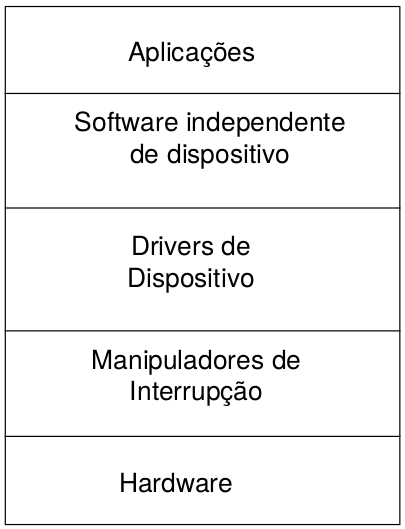
\includegraphics[width=0.35\textwidth]{es-layers}
  \caption{Camadas envolvidas em esquemas de entrada e saída. As camadas 2 à 4 são responsáveis pela gerência de E/S}
  \label{fig:es-layers}
\end{figure}
